\documentclass[tikz,border=10pt]{standalone}
\usetikzlibrary{calc,angles,quotes,intersections}

\begin{document}
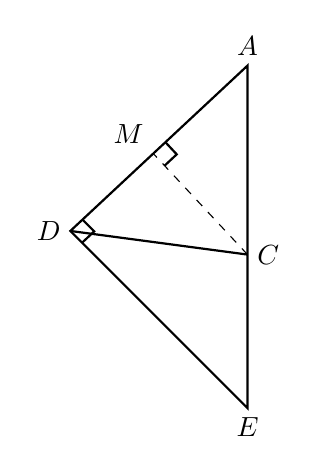
\begin{tikzpicture}[
    scale=1.5,
    important line/.style={thick},
    dashed line/.style={dashed, thin},
    right angle quadrant/.style={draw, thin, minimum size=5pt}
]

    % 1. 定义核心顶点坐标 (基于几何构图比例)
    \coordinate (A) at (0, 2.9);
    \coordinate (E) at (0, 0);
    \coordinate (C) at (0, 1.3); % C点位于AE段上
    \coordinate (D) at (-1.5, 1.5); % D点位置
    
    % 2. 绘制主要实线边界
    \draw[important line] (A) -- (D) -- (E) -- cycle; % 绘制大三角形ADE外框
    \draw[important line] (D) -- (C); % 绘制内连线DC

    % 3. 绘制辅助线 CM (垂直于 AD)
    % 投影点 M 的计算：过C作AD的垂线
    \coordinate (M) at ($(A)!(C)!(D)$);
    \draw[dashed line] (C) -- (M);

    % 4. 绘制直角标记
    % 标记角 ADC 为直角
    \draw[thick] ($(D)!4pt!(A)$) -- ($(D)!4pt!(A)+(D)!4pt!(E)-(D)$) -- ($(D)!4pt!(E)$);
    % 标记角 AMC 为直角
    \draw[thick] ($(M)!4pt!(A)$) -- ($(M)!4pt!(A)+(M)!4pt!(C)-(M)$) -- ($(M)!4pt!(C)$);

    % 5. 标注顶点标签
    \node[above] at (A) {$A$};
    \node[below] at (E) {$E$};
    \node[right] at (C) {$C$};
    \node[left] at (D) {$D$};
    \node[above left] at (M) {$M$};

\end{tikzpicture}
\end{document}